\chapter{An Intertwingled History of Linking}

The act of linking the archive is certainly aided by digital tools, but it is not a requirement. Many indexing and note-taking systems of the Renaissance and Enlightenment allowed for the interlinking of disparate ideas, and these offer useful inspirations and foils for examining the web and its related research tools today. Information overload is not a new phenomenon, and pre-digital knowledge systems had many techniques for what Ann Blair calls the four Ss: storing, summarizing, sorting, and selecting.\autocite[85]{blair_note_2004} Moreover, the web is only one of many digital hypertext systems, and the hyperlink---the primary object and mechanic for network formation on the web---has its own limitations that early hypertextual systems bring into full relief, inviting close analysis of the web's archival affordances.

In Section 2.1 I confessed that my use of the word ``archive'' might expand and contract in scope, signifying a token of preservation and access rather than a singular fixed artifact. In each succeeding section, I aim to hone in my definition of the archive, ultimately to the digital news publishers that form the primary case study of my inquiry. Here my definition remains broad, but I will take a historical rather than theoretical approach to the archive, especially encompassing the pre-digital and pre-web indexes, note-taking systems, bibliographies and encyclopedias that first forayed into networked information.

Most histories of the web's origins begin with Vannevar Bush (and sometimes Paul Otlet before him), leading directly through hypertext pioneers Ted Nelson and Douglas Engelbart, and concluding with Tim Berners-Lee's World Wide Web in a direct line from past to present. I will look closely at these individuals and their goals, and even use this chronological lineage as a structuring point, but I will also break apart this history by introducing other systems and figures---whether they existed long before computers or after the rise of the web---that point towards three corresponding themes. These themes recurrently surface when dealing with digital archives and information management: \emph{spatialization}, \emph{intersubjectivity}, and \emph{encyclopedism}.

\section{Spatialization: The Radiated Library}

Here I will examine the tendency to use visual metaphors for information retrieval, and the associations between memory and physical space. The spatial and dimensional nature of knowledge is at odds with the ``flattening'' effect of indexes and the collapsing of dimensional space that non-hierarchical linking affords. Cycling through Ephraim Chambers' \emph{Cyclopaedia}, I will examine Paul Otlet's vision of the ``radiated library'' and his architectural inspirations.

Memory has a strong spatial component; even when we don't remember something, we often know where to find it. A 2011 Columbia University study asked participants to save statements into various folders with generic names (such as FACTS, DATA, INFO, and POINTS). Despite the unmemorable folder names, ``participants recalled the places where the statements were kept better than they recalled the statements themselves.'' The researchers found that ``\thinspace `where' was prioritized in memory,'' providing preliminary evidence that people ``are more likely to remember where to find it than to remember the details of the item.''\autocite{sparrow_google_2011} They conclude by suggesting that we may be using Google and Wikipedia as memory extensions that then rewire our own internal memory.

But humans have relied on external memory since the origin of writing itself, and in the meantime we have developed scores of analog systems and techniques---Barnet might call them ``memory machines,'' John Willinsky ``technologies of knowing''---to help summarize, filter, sort, and select. Computer systems are only one piece of this longer history of tools and practices. David Weinberger's ``three orders of order'' suggest this continuum, while also pointing out the rupture that the digital creates. The first order consists of things themselves, such as books in a library. The second order is a physical set of indexes, pointers, and references to the things, like a library card catalog. Finally, the third order is the digital reference, made of bits instead of atoms.\autocite[17-23]{weinberger_everything_2008} The third order allows items to be in multiple categories at once, as if in multiple sections of the library---this is a phenomenon that information architects call \emph{polyhierarchy}.

A theme across all of these orders of order is a reliance on spatial memory (the ``where to find it'' in the Columbia study). Archival and classification schemes use terms like ``border,'' ``domain,'' and ``kingdom'' (is it a coincidence that these terms all carry connotations of politics and power struggle?). We visualize network schemes as trees and as rhizomes, represented on maps, graphs, and diagrams. It seems that proper spatial visualization of an archive might not only help us remember where something is saved, but also give a high-level understanding of the archive itself, improving browsing and serendipitous search.

The ancient practice of constructing ``memory palaces'' (and Giulio Camillo's memory theater of the Renaissance)---outlined in Frances Yates' \emph{The Art of Memory}---strongly emphasizes memory's reliance on spatial orientation and fixed dimension.\autocite{yates_art_1966} In order to construct a memory palace, the first step is to imagine a series of \emph{loci}, or places, to determine the order of the facts. Only after creating space can one then create the images that represent the facts themselves. The structure that these palaces take on are up to the memorizer, but once fixed, they are rarely reordered---only added to. This completes a grander spatial metaphor that Peter Burke notices---that of the \emph{course}, which a student must run, envisioning and memorizing \emph{images} in \emph{places} along the fixed route towards knowledge.\autocite[90]{burke_social_2000} Such an exercise emphasizes the temporal as well as spatial, as items are better remembered in sequence (such as with a rhyming poem).

This reliance on spatial and temporal memory keeps us in just two or three dimensions; it does not escape the trappings of the physical archive. If our memories rely on a fixed visual referent to know where a book is in a library, then we cannot rearrange the library's stacks and expect to find it again. A similar concern arises with online reading and writing. Ted Nelson calls hypertext ``multi-dimensional,'' and Stuart Moulthrop says it aims to be ``writing in a higher-dimensional space,''\autocite{barnet_mandelbrot_2013} but some readers still prefer paper-imitating PDFs to websites and e-books, because PDFs maintain a layer of real-world dimensional reference (as in, ``I remember reading that sentence near the top of the page in the left column\ldots''). For all of the liberating power of the digital, computers still rely on physical metaphors to be usable, and so we use digital equivalents of desktops, files, folders, and cards. The web even nods to this with its hierarchical URL structure that asks us to ``navigate'' down ``paths'' in given ``domains.''

This last fact is surprising given that a common theme among hypertext's pioneers, including Berners-Lee, is a desire to break down traditional linear and hierarchical classification schemes. A hierarchical scheme---like Linnaeus's biological taxonomy or Dewey's decimal classification---immediately suggests a tree view, and we can find many old examples of tree graphs in the Renaissance and Enlightenment. On the other hand, an alphabetical scheme offers a linear view, one that flattens the brittle hierarchy of taxonomy, but dulls its potential for association. The linked hypertext view might be seen as a multi-dimensional graph, more nuanced and flexible but more difficult to grasp. If the first two orders are in one (linear) and two (hierarchical) dimensions, how can we bring the third order of order into a still higher dimension? And can it complement the ways that our minds visualize information?

\subsection{The linked encyclopedia}

Some older, pre-digital systems and practices have hybrid hierarchical/linear structures that start to suggest a network. While not the first system to incorporate links, Ephraim Chambers' \emph{Cyclopaedia} is one of the first reference works of its kind. The encyclopedia reads somewhat like a dictionary, but it expands into general knowledge and opinion as well, and it always suggests multiple views into its contents. Chambers wrote that his encyclopedia went beyond a dictionary because it was ``capable of the advantages of a continued discourse.''\autocites[i]{chambers_cyclopaedia_1728}[64]{yeo_solution_2003} The word ``encyclopedia'' literally means ``circle of learning,'' calling into question the shape of such a knowledge structure. It may be organized linearly, but as a collection of words to describe words, it always strives to double back on itself and highlight its own circular logic.

\begin{figure}[ht]
\centering
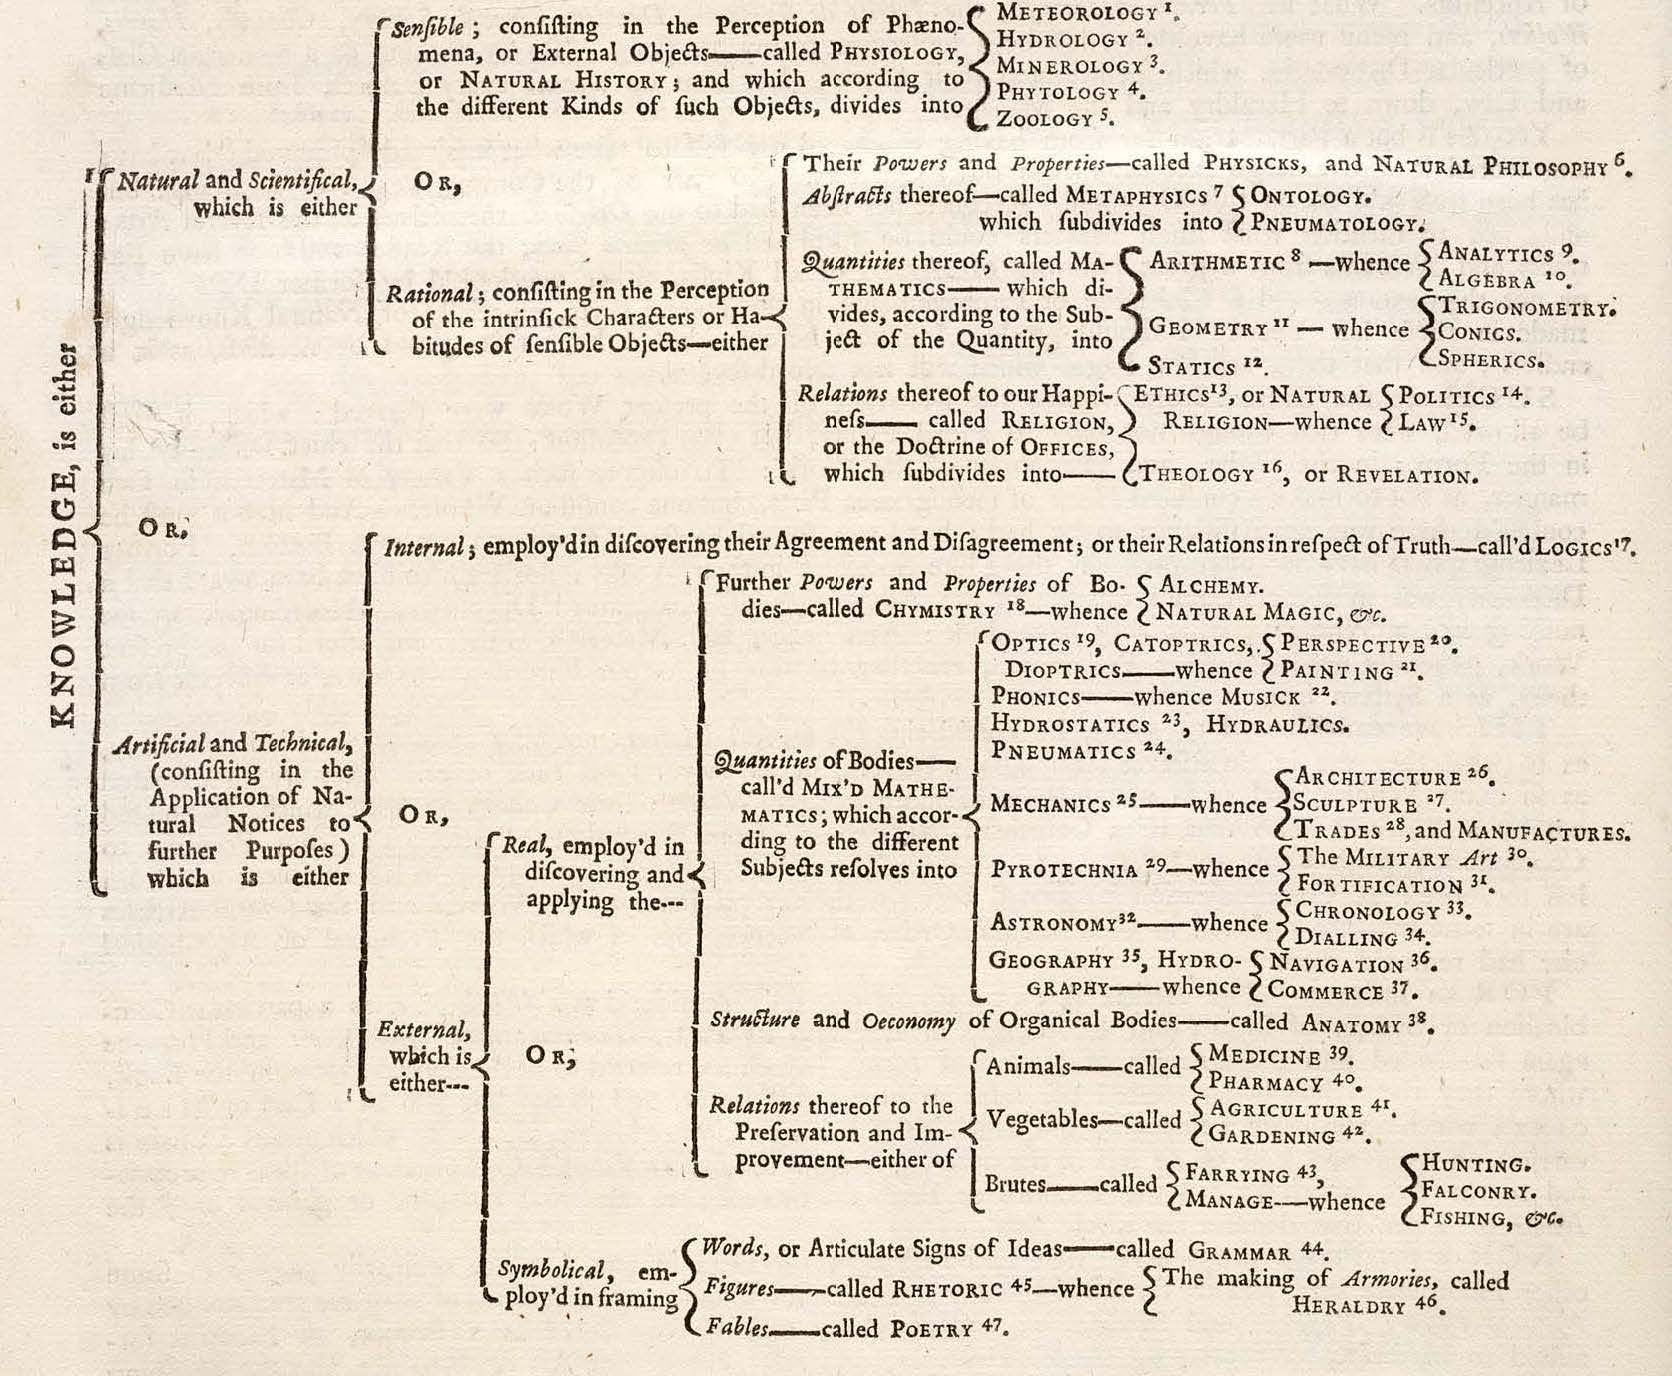
\includegraphics[width=400pt]{figures/cyclopaedia-tree}
\caption{The ``branches of knowledge'' in Ephraim Chambers' \emph{Cyclopaedia}.}
\label{fig:cyclopaedia-tree}
\end{figure}

The \emph{Cyclopaedia} was organized alphabetically, a relatively bold form of classification in relationship to the traditional, hierarchical schemes. Most scholars seem to agree that alphabetical order was born out of sheer necessity, related to the ``intellectual entropy'' and ``epistemological urgency'' of the time.\autocite[5]{rosenberg_early_2003} New knowledge was simply being created too fast to systematize and order. But Michael Zimmer suggests that alphabetical order signaled the beginning of a shift to more distributed, networked, and ``egalitarian'' forms of knowledge organization.\autocite[100]{zimmer_renvois_2009} For instance, religious topics would be placed alongside secular ones. Alphabetical organization also turned the system into more of a ``quick reference'' guide that favored brief digests over long forays into knowledge; the practices of browsing, skimming and summarizing were continuously honed during the Renaissance and Enlightenment as scholars coped with ``a confusing and harmful abundance of books'' as early as 1545.\autocite{blair_reading_2003} Chambers called this complaint ``as old as Solomon.''\autocite[65]{yeo_solution_2003}

All the same, Chambers felt he needed an overarching scheme. In the encyclopedia's preface, he included a diagram and listing of forty-seven categories (called Heads), complete with cross-references to the entries. In Chambers' words, ``the difficulty lay in the form and oeconomy of it; so to dispose such a multitude of materials, as not to make a confused heap of incoherent Parts, but one consistent Whole.''\autocite[67]{yeo_solution_2003} In order to truly demonstrate a ``continued discourse,'' Chambers needed a graph, a map. Each of the Heads in the diagram contains a footnote that lists that head's terms (known as Common Places).\footnote{(add more historical diagrams of graphs, trees, maps)}

Chambers' use of Heads and Common Places followed Phillipp Melanchthon's 1521 subject division into \emph{loci} and \emph{capita} (Peter Burke suggests that these would now be called ``topics'' and ``headings,'' less strong and physical metaphors).\autocite[95]{burke_social_2000} \emph{Loci} (``places'') bring to mind memory palaces, but also the ``commonplace book''---to which Chambers was knowingly attaching himself. Many scholars used commonplace books as information management devices to store quotes, summaries, aphorisms, and so on, and these often had specialized systems for retrieval. Richard Yeo sees Chambers' use of the term as directly appealing to the popularity of commonplace books at the time.\autocite[65-66]{yeo_solution_2003} Ann Blair also argues that note-taking and commonplacing were far more common than the memory palaces and theaters outlined by Frances Yates, and that the two traditions made ``no explicit reference to one another.''\autocite[``Note Taking as an Aid to Memory'']{blair_too_2010} Still they share a strong common thread: a reliance on \emph{loci} as the root of knowledge retention, memory, and interconnection.

The \emph{Cyclopaedia} was an ancestor to Diderot's celebrated \emph{Encyclop\'{e}die} (Diderot started by translating Chambers). Diderot's work made further use of \emph{renvois} (references) to question and subvert traditional knowledge structures and authorities---including the book's own authority as a reference work. Michael Zimmer argues that Diderot also used \emph{renvois} to hide politically controversial topics in seemingly dry and tangential entries, ``guiding the reader to radical or subversive knowledge'' while evading the eyes of the censors.\autocite[103]{zimmer_renvois_2009} Zimmer directly ties the \emph{renvois} to the hypertext link, suggesting that Bush, Nelson, and Berners-Lee all ``intended to free users from the hegemony of fixed information organization in much the same way that \emph{renvois} did for the readers of the \emph{Encyclop\'{e}die}.''\autocite[104]{zimmer_renvois_2009}

\begin{figure}[ht]
\centering
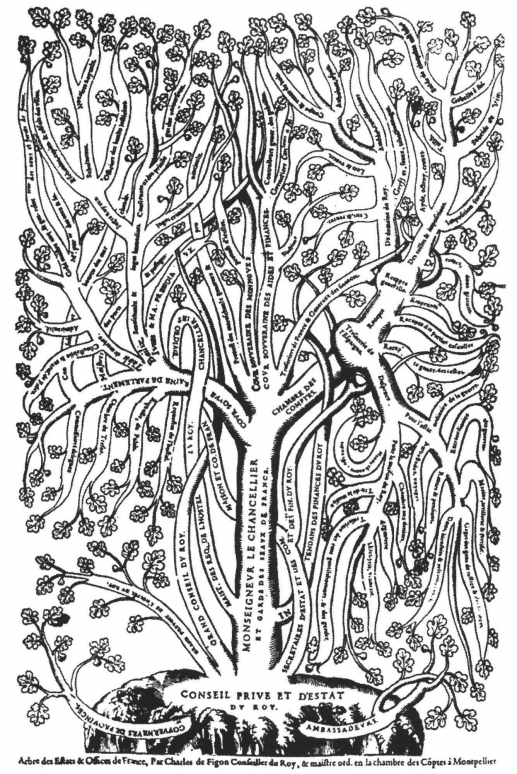
\includegraphics[height=400pt]{figures/historictree}
\caption{Arbre des Etats et Offices de France, by Charles de Figon (Paris 1579).}
\label{fig:historictree}
\end{figure}

It is clear that Diderot fully recognized and built upon Chambers' developments in linking references, but I call into question the notion that the prior ``fixed'' organization systems had no detractors or provisional solutions (moreover, the \emph{renvois} are ``fixed'' themselves). Carolus Linnaeus, the author of perhaps \emph{the} prototypical taxonomy, knew well that classifications are ``cultural constructs reflecting human ignorance.''\autocite[99]{zimmer_renvois_2009} Leibniz also understood its limitations; his \emph{Plan for Arranging a Library} included a ``miscellaneous'' section, a tacit acknowledgement that the system is in some way imperfect or incomplete.\autocite[106]{burke_social_2000} Leibniz also praised his famous Note Closet, developed by Thomas Harrison, for this same ability: ``A single truth can usually be put in different places, according to the various terms it contains\ldots and different matters to which it is relevant.''\autocite[``Managing Abundant Notes'']{blair_too_2010}

Moreover, multiple hierarchies can coexist and offer competing schemes. Some of these schemes were already organized not as much around content as con\emph{text}. Peter Burke points out that Islamic classification systems were also tree-structured, but every element was organized based on its degree of separation from the Quran.\autocite[94]{burke_social_2000} This is, crucially, an early citation-based network.

\subsection{Paul Otlet and the dimensions of memory}

Along with Vannevar Bush, Paul Otlet bridges the second and third orders of order. Born in Belgium in 1868, Otlet predated Ted Nelson's role as an obsessive encyclopedist and commonplacer. Between the ages of ages 11 and 27, he amassed 1400 pages of notes, and in his first move to Paris, he called it ``the city where the world comes to take notes.''\autocite{_limited_2001}  He liked to think big and in the aggregate, creating the Universal Decimal Classification and Universal Bibliographic Repertory. He also supported international politics associations like the League of Nations and the forerunner to UNESCO, going so far as to found the Union of International Assocations (which is, indeed, an international association of international associations) with his friend Henri La Fontaine in 1907.

Due in part to the destruction of much of his work in World War II, Otlet was mostly forgotten for decades in favor of his American successors. However, the rise of the web and the efforts of several scholars---particularly his biographer Boyd Rayward---have given him a new life as a prescient predictor of a networked hypertext system. As one of the originators of information science, he envisioned (and even began to amass) a universal library to serve as the heart and central authority of the world's information. Following his belief that books were redundant and arbitrary agglomerations that obscure the data held within (which is the object of a researcher's true inquiry), he suggested a universal decimal classification system that built on Dewey's system to incorporate an item's metadata, its references and constituent parts. Its entries read less like library call numbers and more like modern databases' structured queries. And in his most striking prediction, he proposed a ``radiated library'' that could handle remote requests from a centralized location by screen and telephone. He envisioned the screen with multiple windows for simultaneous document consultation, audiovisual data, and finally a full automation of the document request process: ``Cinema, phonographs, radio, television, these instruments taken as substitutes for the book, will in fact become the new book.''\autocite{van_veelen_alle_1998} Otlet's ``radiated library'' and ``televised book'' combine to suggest the networked multimedia of the web, more than 50 years before its creation.

\begin{figure}[ht]
\centering
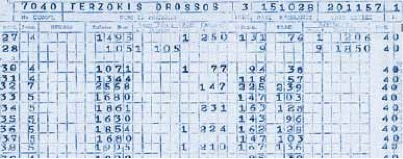
\includegraphics[width=300pt]{figures/otlet}
\caption{Excerpt of the Universal Library's indexing system.}
\label{fig:otlet}
\end{figure}

Otlet was an encyclopedist, but also an innovator in graphical and spatial representation. He frequently used architecture as a foil, metaphor, and inspiration for bibliographic structures, calling his main work \emph{Trait\'{e} de documentation} a study of the ``architecture of ideas.''\autocite[129]{van_de_heuvel_building_2008} The first names for the Mundaneum---the universal repository Otlet and La Fontaine set out to build---were alternately ``city of knowledge'' and ``World Palace.'' In the end, the Mundaneum---like the archive itself---bridged the physical and the digital or metaphysical, as Otlet called it at once ``an idea, an institution, a method, a material body of work, a building and a network.''\autocite[130]{van_de_heuvel_building_2008} In his discussion of the architecting of knowledge, Otlet also crucially recognized that ideas are never so fixed as physical structures; as Charles van de Heuvel puts it, ``For Otlet it was important to leave space for transformation and modification in response to the unforeseen and unpredictable.''\autocite[131]{van_de_heuvel_building_2008} Leibniz had conceived of the ``library without walls'' long before, but Otlet's radiated library went many steps further. As one of the fathers of information science, he is also one of its first information architects.

Otlet's resulting decimal classification and networked library is less bound by linear or hierarchical schemes. The architectural inspiration also may have helped him conceive of the radiated library, one that could transmit signals across space between screens, several decades before the first computers were linked together. All the same, it is hard to see Otlet's universal library project as anything but quixotic. The perpetual collection and detailed organization of the entirety of human history in one location, all managed by 3x5 index cards, is doomed to fail. Still, Otlet's system seems to have worked usefully for a time: the library had more than 17 million entries by 1934, handling 1500 research requests per year, all on the backbone of Otlet's Universal Decimal Classification.\autocite{_limited_2001} The universal repository was, of course, never completed, but it came closer to fruition than the memex or Xanadu.

% Talk about videotheque?

\section{Intersubjectivity: The Memex}

An individual's personal archive has markedly different properties and requirements than a group's or institution's, which in turn is different from a massive, aggregated universal archive for the public. At the same time, some archives sit in between these scopes, and each has different purposes and practices surrounding it. Linking and categorization schemes rely on individuals making connections between information, but different individuals might not make the same connections; how does linking become a collective and collaborative endeavor, a universal language? This phenomenon is both explicated and emphasized by a contemporary example: the web's algorithmic recommendation systems that conflate the individual and the collective as they traverse the links of the web.

The scrapbooks, commonplace books, and card catalogs of old usually belonged to an individual. He or she might share them and collaborate with others, or collect resources for children and grandchildren, but these early systems generally reflected and mimicked the scattered mind of a single person. A scholar's notes are likely to consist of many shorthands, mental leaps, and personal anecdotes that no one else would follow. Interestingly, most early hypertext systems focused on this individual scope, or at most on collaborative or collective research. Only Xanadu (and perhaps Otlet's Mundaneum) had the world-encompassing scope of the web.

Jeremias Drexel stated in 1638 that there is no substitute for personal note-taking: ``One's own notes are the best notes. One page of excerpts written by your own labor will be of greater use to you than ten, even twenty or one hundred pages made by the diligence of another.''\autocite{blair_note_2004} People forge connections and organizational schemes in unique and sometimes conflicting ways. As more and more people enter a system, it will encounter more and more possible definitions and connections.

The idiosyncratic connections formed by an individual's memory make it difficult to generalize categories. An individual's thought process might be reminiscent of Borges' Chinese encyclopedia, which offers a taxonomy of animals divided by absurd traits, such as ``Those that belong to the emperor, embalmed ones, those that are trained, suckling pigs, mermaids, fabulous ones, stray dogs,'' and ``those that are included in this classification.''\autocite{borges_analytical_1993} These may be the trails that a mind follows, but the humor lies in calling it a taxonomy, in making the categories \emph{intersubjective} and even official, \emph{objective}. Borges' categories remind us of Bowker and Star's argument that classifications will always be compromises, between individuals and groups, or between groups and a collective whole.

Markus Krajewski's \emph{Paper Machines: About Cards and Catalogs} hinges on the difference and tension between a personal note-taking system and a universal library. We often use the same systems for organizing each (such as the card catalog or the SQL database), but they don't turn out to be for the same uses. Krajewski says ``The difference between the collective search engine and the learned box of paper slips lies in its contingency.''\autocite[50]{krajewski_paper_2011} Whenever we add a tag or make a connection in an archive, we are attempting to predict what will be searched for later. But it is easier to classify in a personal archive; we can predict our future selves better than we can predict the future.

As a result, personal note-taking tools might seem like an easier place to start with the challenge of hypertext. They are certainly technically easier, avoiding collaboration issues like version control. But an archive is almost never entirely personal. Thought may be idiosyncratic, but it follows common patterns. Users want the possibility of sharing documents, or of passing on entire collections to others. Ann Blair points out that successors would fight over their ancestors' notes in Renaissance wills, which suggests that any time a commonplace book is begun, it has some kind of common value.\autocite[104]{blair_note_2004} In the case of historical figures, personal notes often become a literal part of an archive, then meant for public consultation. But we treat these archives differently than those that are constructed \emph{for} us. For instance, Walter Benjamin's \emph{Arcades Project} is a set of notecards, published as a sort of commonplace book that has become a prominent work to consult in its own right. Is it a book, an archive, or a database? Who is it for? What happens to Benjamin's memory as it becomes shared history?

This relationship between the personal and the collective is taking on new meaning on the web, where we expect personalized information, but rely on a massive collective of people in order to get it. Nick Seaver argues that recommendation systems ``algorithmically rearticulate the relationship between individual and aggregate traits.''\autocite{seaver_algorithmic_2012} The communities and demographics that form around individuals can in turn be aggregated and intersected into a single, massive whole. At each stage, memory is abstracted further and further from us.

Today's efforts to organize the web and its sub-archives (i.e. the web applications, tools, and platforms we use every day) tend to reflect this and aim to marry the best of both worlds: the individual and the mass. Clay Shirky and David Weinberger champion the folksonomy as a solution; let individuals tag however they want, and at the right scale everything will sort itself out.\autocites{shirky_ontology_2005}[165-8]{weinberger_everything_2008} The Semantic Web is similarly structured, by letting users define their own vocabularies for both pages and links, but strictly enforcing them once made.  These approaches are certainly worth pursuing, but both still rely on fixed language rather than associative connection; tagging an item is undoubtedly an act meant to make connections between documents, but it is always mediated by language and structured according to certain systematic and linguistic conventions.

\subsection{Vannevar Bush's memory machine}

Unlike Otlet's radiated library, or Nelson's Xanadu, Vannevar Bush's memex was decidedly a machine designed for personal use. It did not build in weblike networked affordances. All the same, Bush suggests many intersubjective uses for the memex, adding to the confusion between personal archive and collective library.

Bush was perhaps best known as the director of U.S. military research and development during World War II, but he also made a lasting contribution to hypertext; a 1945 essay called ``As We May Think'' conceived of the memex machine, an automated microfilm device that could store an entire library in one drawer and retrieve any item within seconds.\autocite{bush_as_1945} Perhaps most crucially, Bush conceived of new ways to connect items: through associative trails. Linda C. Smith analyzed the citation network of many hypertext articles and discovered, in Belinda Barnet's words, that ``there is a conviction, without dissent, that modern hypertext is traceable to this article.''\autocite{barnet_technical_2008}

Bush begins by arguing that, ``The summation of human experience is being expanded at a prodigious rate,'' but suggests that our methods for retrieving such experience are hindered by ``the artificiality of systems of indexing.''\autocite{bush_as_1945} He points out the limitations of keeping data only in one place, and of using strict formal rules to access it: ``the human mind does not work that way. It operates by association. With one item in its grasp, it snaps instantly to the next that is suggested by the association of thoughts, in accordance with some intricate web of trails carried by the cells of the brain.'' His proposed solution, the memex, aims to mechanize ``selection by association, rather than by indexing.''\autocite{bush_as_1945}

The memex is built for personal use; Bush's model is ``the human mind,'' after all, and not ``human minds'' (as Barnet notes, he follows the cybernetic tradition of the time in modeling computation on human thought, along with Wiener, Shannon, Licklider, and others).\autocite{barnet_technical_2008} The idiosyncrasies of individual trails, and the challenges in developing a new language for a new invention, would suggest that the machine was strictly for individual use. However, Bush points immediately to its possibility for generalization as well; he envisions an example of a person sending his trail of research to a colleague ``for insertion in his own memex, there to be linked into the more general trail.''\autocite{bush_as_1945}

\begin{figure}[ht]
\centering
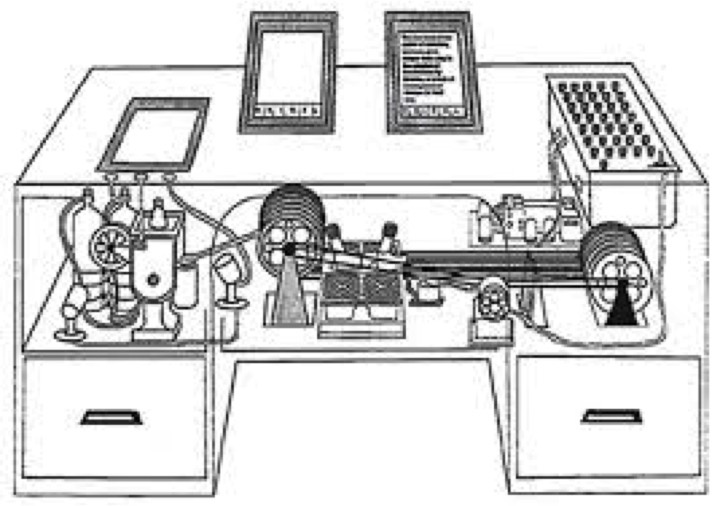
\includegraphics[width=350pt]{figures/memex}
\caption{Vannevar Bush's memex diagram.}
\label{fig:memex}
\end{figure}

Bush goes on to suggest that the memex will hold new forms of encyclopedias and ready-made trails, along with ``a new profession of trail blazers, those who find delight in the task of establishing useful trails through the enormous mass of the common record.''\autocite{bush_as_1945} This now seems prophetic, a prediction of contemporary culture's emphasis on curation, though it was predated by Otlet's assertion that we will need a new class of ``readers, abstractors, systematisers, abbreviators, summarizers and ultimately synthesizers.''\autocite[23]{reagle_good_2010} Bush does not dwell on this to consider where this ``common record'' will live, who will own and control it, and how individuals will tie these resources to their own idiosyncratic trails. The shift from subjectivity to intersubjectivity, and then in turn from intersubjectivity to some form of \emph{objectivity}, makes each act of classification---or in Bush's case, each act of association---increasingly fraught.

Bush's work relies on the trail, a closely curated path where one document directly associates with another. Ted Nelson instead suggested ``zippered lists,'' which would operate like trails but without Bush's emphasis on sequence.\autocite[84, 89]{nelson_complex_1965} In each of these cases they rely on a human curator to create the links. Bush envisions trails shared for personal, collaborative, and general use, but the connection itself remains person-to-person, intersubjective on the smallest scale. The trails and associations formed by the memex always remain deeply human, and deeply individual.

In Bush's ``Memex Revisited,'' he begins to tease out the possibility of the memex forming trails for a scholar, suggesting that it could ``learn from its own experience and to refine its own trails.''\autocite[211]{bush_memex_1991} Here the influence of Wiener's cybernetics and feedback theory are clear, and it begins to point to the machine learning and automated classification that occurs today. Most intriguing is Bush's suggestion that like the human mind, some well-worn trails would be kept in memory, reinforced and expanded, while other less-used trails would fall away. This conjures up the notion of a fluid archive, one that is constantly forming and re-forming its associations, dynamically linking the past.

But Bush's memex is not without its limitations. John H. Weakland offered two criticisms of the memex in response to ``As We May Think.'' He asks ``how personal associations of the general record could be generally useful,'' as well as how a researcher can find things they don't know about already.\autocite[217]{nyce_innovation_1989} It appears to me that the second challenge is an extension of the first: associative indexing may be more inherently fuzzy and idiosyncratic than content-based indexing systems like text search and tagging. It sacrifices fixity and consistency at the expense of individuality and nuance.

Another limitation of the memex, offered by Belinda Barnet, is that ``Bush's model of mental association was itself technological; the mind `snapped' between allied items, an unconscious movement directed by the trails themselves.''\autocite{barnet_technical_2008} Bush himself recognized this, pointing out that the human memory system is a ``three-dimensional array of cells'' that can gather, re-form, and select relationships as a whole or a subset of a whole.\autocite[209]{bush_memex_1991} While later hypertext systems and the Semantic Web come closer to such a three-dimensional structure, like the memex they are often constrained to `snapping' between associations.

Finally, even though Bush seems fully aware of the morphing state of collective knowledge and history, he assumed that the trails would not grow old. He envisions a father bequeathing a memex to his son, along with the myriad trails formed, as a fixed and locked document. Even Bush's proposed adaptive memex would be modeled against the individual researcher; in machine learning terms, its ``training set'' would not be formed in the aggregate like modern-day recommendation systems, but rather from the unique trails formed by an individual.

\section{Encyclopedism: Project Xanadu}

This section analyzes the scale of knowledge systems, and specifically the constant striving to expand beyond the archive's horizon. While the last section was based on the type and scale of \emph{users} of the archive, this section concerns the type and scale of \emph{information} or \emph{content} within the archive. There does tend to be a relationship---an archive built for everyone is more likely to collect everything---but I divide them here to highlight the tendency for content to stretch towards complete and total comprehensiveness, or what I am calling \emph{encyclopedism}. Many efforts to document, index, or link the world have truly attempted to map \emph{the world}---every piece of information about everything---or have at least appealed to an impulse to do so. What leads to this encyclopedic impulse, and what are some of its promises and pitfalls? When building an archive, where do you stop?

Paul Otlet wanted to index all of every book. In his notes, he insists, ``I write down everything that goes through my mind, but none of it has a sequel. At the moment there is only one thing I must do! That is, to gather together my material of all kinds, and connect it with everything else I have done up till now.''\autocite[20]{reagle_good_2010} This persistent, obsessive quest for comprehensiveness is part and parcel of the archive---you either want to collect and connect \emph{everything}, or everything \emph{worthwhile}, within a given scope.

Once again this conjures up a Borges story: his Library of Babel contains books with every permutation and combination of every letter. \emph{Somewhere} in the library sits every great work ever written, and every great work that will be written. But the vast majority of these books are useless nonsense, and no great works will be found. Borges, a librarian himself, understood well the encyclopedic impulse and the noise and madness that results.\autocite[112-18]{borges_collected_1999}

Encyclopedism has its roots at least in the Renaissance, as Ann Blair notes: ``it is reasonable to speak of encyclopedic ambition as a central ingredient of the Renaissance obsession with accumulating information.''\autocite[``Information Management in Comparative Perspective'']{blair_too_2010} Even in 1548, Conrad Gesner began compiling a ``general bibliography'' with the aim of indexing all known books; he ended with 10,000 works by 3,000 authors, which was surely an obsolete number even by the time he finished.\autocite[93]{burke_social_2000} Some critics, like Jesuit scholars Francesco Sacchini and Antonio Possevino, recommended an ``aggressively purged'' rather than universal library, throwing out any redundant or misleading texts. Gesner disagreed, but his reasoning was telling: ``No author was spurned by me, not so much because I considered them all worthy of being cataloged or remembered, but rather to satisfy the plan which I had set for myself.''\autocite[``Bibliographies'']{blair_too_2010} He wanted to list all the books in order to leave others to be the judge, but first and foremost, he did it because it was his plan all along.

Some of today's technological language reflects this drive. Wikipedia's mission is ``to give freely the sum of the world's knowledge to every single person on the planet,''\autocite[18]{reagle_good_2010} which is reminiscent of Google's: ``to organize the world's information and make it universally accessible and useful.''\autocite{_company_????} The \emph{world's} knowledge, \emph{universally} accessible, to \emph{every} person: the goal is impossible. Capturing ``the sum of the world's knowledge'' is akin to Borges' aleph---a point that contains all points---or his one-to-one map of the world. Still, Wikipedia knows well that ``Regretfully, the vast majority of human knowledge is not, in actual fact, of interest to anyone, and the benefit of recording this collective total is dubious at best.''\autocite[17]{reagle_good_2010}

All of these universal projects are destined to fail at their end goal, but the resulting collections can be useful. The book repositories and knowledge systems of today---Wikipedia, Google Books, Project Gutenberg, and Amazon---may have come closer than any previous efforts to capturing the world's knowledge, but they do so according to certain principles, conventions, demands and traditions. They also have something else in common: they must always adhere to the technical and conventional standards and limitations of the web itself. 

\subsection{Ted Nelson's endless archive}

Ted Nelson, inventor of the term ``hypertext,'' is a notorious collector, commonplacer, and self-documenter. He also always thinks big; he wants to collect \emph{everything} and connect \emph{everything} to \emph{everything} (``everything is intertwingled,'' in his parlance), and only then will it all make sense. His project for doing so, called Xanadu, began work in 1960 and has inspired scores of hypertext acolytes, but after so many years of continuous development, it still has not been fully realized.

Nelson was deeply inspired by Bush's memex, referencing him frequently in presentations and even including the entirety of ``As We May Think'' in his book \emph{Literary Machines}. Building on Bush's ideas, Nelson suggested ``zippered lists'' instead of trails, which could be linked or unliked as its creator desired, advancing beyond Bush's ``prearranged sequences.''\autocite[313]{nelson_computer_1974} But his biggest development was to reintroduce the global ambition of Otlet into Bush's associative vision: the idea of a universal, networked, collectively managed hypertext system.

\begin{figure}[ht]
\centering
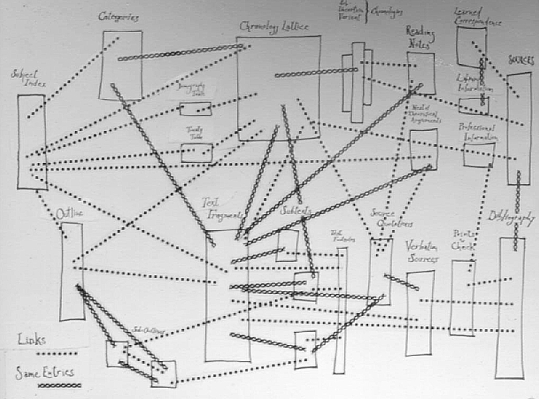
\includegraphics[width=350pt]{figures/xanadu}
\caption{Schematic of a sample linked system in Xanadu.}
\label{fig:xanadu}
\end{figure}

In Nelson's system, there would be no 404s, no missing links, no changes to pages forever lost to history. Links would be two-way, forged in both directions---imagine visiting a page and being able to immediately consult every page that linked \emph{to} the page. And rather than copying, Xanadu operates on \emph{transclusion}, a sort of soft link or window between documents that would allow new items to be quickly and easily constructed from constituent parts, readily pointing back to their source.

Nelson's idea for Xanadu might resemble Wikipedia; one of Wikipedia's core tenets is ``No Original Research: don't create anything from scratch, just compile,'' reflecting the principle of Nelson's transclusions.\autocite[11-12]{reagle_good_2010} But on the web, where so much information is ripe for mash-up, remix, and reuse, the only option is to create from scratch. The links at the footer or the inside of a Wikipedia page are merely pointers and not true windows into the source documents. Nelson's transclusions are more akin to the Windows shortcut, Mac alias, or Linux softlink. The Web's default, on the other hand, is to \emph{copy} rather than \emph{link}. Jaron Lanier suggests that copying-not-linking is a vestige of the personal computer's origins at Xerox PARC, whose employer was quite literally in the business of copying, and was inherently wary of ideas that bypassed it.\autocite[221-232]{lanier_who_2013}

One could look at the resulting Wikipedia, or any such aggregation of compiled knowledge, as a combination of two actions: \emph{summarizing} and \emph{filtering}. To summarize is to provide a shorter version of a longer text. To filter is to offer a verbatim excerpt of the text. Most knowledge systems that I am addressing here exist along a continuum between these two primary actions, and effective ones are able to elegantly balance both. Xanadu places more focus on filtering texts, while the web might lend itself better to summarizing; it is only through the web's hyperlinks that we get a glimpse of a filtering axis.

But unlike the web, Xanadu has still not been fully realized. It has lost, while the web has experienced an unprecedented, meteoric rise. Xanadu also has its share of detractors and challengers. Most of its biographies and summaries are fairly critical, most famously a 1995 \emph{Wired} article that prompted a forceful response from Nelson.\autocite{wolf_curse_1995} There is a level of hubris in the encyclopedic impulse that Nelson doesn't hide. His proposed system is top-down and brittle in certain ways, including rigid security and identification systems. And his proposal for online ``micropayments'' per transclusion is interesting but controversial; Jaron Lanier and others have supported it, but many are skeptical, suggesting that it would stifle the sharing of knowledge and circulation of material.\autocites{atwood_xanadu_2009}[Chapter 18]{lanier_who_2013}

The Xanadu system is far from perfect, but its allure comes from the idea that it treats its contents with history and context in mind. Xanadu promised to treat its contents like an archive rather than making us build archives around it. Comparing it to the web raises interesting questions: how much structure, organization, and control should we place on our networked information systems? How much is desirable, and how much is technically and economically feasible? And if we consider the archival capabilities of each, how are they building, sorting, and selecting our information?

A skeletal version of Xanadu (still \emph{without} its two-way links) was finally released on the web, after more than 50 years of development, in summer 2014.\autocites{carmody_pioneering_2014}{hern_worlds_2014} It has joined the myriad archives and knowledge systems embedded inside the web. Many of the later, ``second-generation'' hypertext systems were geared towards personal and institutional uses (systems like NoteCards, Guide, WE, or Apple's HyperCard).\autocite{halasz_reflections_1988} These likewise resemble the web platforms and tools we use today (such as Trello, Evernote, or Zotero). But these systems, like Xanadu itself, have been subsumed by the web. Hypertext systems can all interact with one another, but the encyclopedic, universal ones can only be in competition.

\section{Conclusion}

This long history of linked, indexed, and sorted archives would suggest that the current state of archives in the digital era has occurred as a result of a continuum of developments, rather than a radical leap into completely unknown territory. But in another sense, the digital does allow for a complete rupture. The ``information overload'' we experience today is a product of two factors, one old and one new. The \emph{accumulation} of the archive is an age-old challenge that many tools, systems and practices have endeavored to solve. But the \emph{linking} of the archive is a newer challenge. There has always been too much information, but now it can all be connected, quantified, broken down and aggregated as never before. As we sort through the webbed intersections of content and context, it will be crucial to keep in mind its long history; after all, it is what archives are fighting to preserve.

Archives' constant battle with issues of scope and dimensionality suggest a need to recognize and limit ambitions, to start small and build up rather than starting from the whole and breaking down. The linking of the archive requires knowing your archive---who is it for? How big is it, and how big do you want it to be? What visual and dimensional language can you employ to help the user navigate?

Looking to history can also temper the conclusions we attempt to draw from archives. The web's massive structure suggests total comprehensiveness---a true universal library---and understanding the limits of its scope \emph{as well as} the limits of its context allows us to view its contents with greater nuance. This is a crucial question as our linked archives begin to link with one another, such as with linked data and APIs. These create new modes of analysis that suggest an inarguable universality: as danah boyd and Kate Crawford argue, ``Big Data reframes key questions about the constitution of knowledge, the processes of research, how we should engage with information, and the nature and the categorization of reality.''\autocite{crawford_critical_2012} A full understanding of the structures and challenges in network- and archive-building gives us one view into what boyd and Crawford call the ``models of intelligibility'' and ``inbuilt limitations'' of big data itself.

The web has evolved since its inception to support much more complex applications, structures, and graphics. But any new developments and platforms must be grafted onto the web rather than rethinking its core structure. I have aimed to suggest how historical context and understanding of the challenges and structures of early hypertext and information management systems can help to explain the powers and limitations of the web. These knowledge systems can also provide inspiration for new solutions: web-based digital archives could aim to mimic or approximate multiple linking, transclusions, or high-level graph views, all while keeping in mind their respective archive's size, shape, and scope.
